Eine Klassifikation ist dann, wenn ein NN eingegebene Daten zu 
    eindeutigen Klassen zuordnen soll.

\section{Quellen für Programmierung}
keras.io, numpy.org, stackoverflow, discuss.pytorch.org, pytorch.org, kaggle

\section{Beschreibung der Tätigkeit}
    
    Es soll TF mit Klassifikation durchgeführt werden. 
    Genutzt wird hier ein Domainwechsel, da die Datensätze gewechselt werden. 
    Die dafür vorgesehenen Datensätze sind Modified National Institute of 
    Standards and Technology(MNIST) und Streetview House Numbers(SVHN). 
    Es gibt die Frameworks PyTorch und Keras, die ebenfalls miteinander 
    verglichen werden. 
    Der MNIST-Datensatz ist dabei die Source und der SVHN das Target. 
    Um einen Vergleichswert zu haben, wurden beide Netze auch allein gelöst. 
    
\section{Ergebnisse PyTorch}
    MNIST ist sehr leicht zu lösen. Es reicht ein einzelnes Linearlayer bei keiner expliziten
    Aktivierungsfunktion. Softmax wird automatisch von PyTorch hinzugefügt. 
    Dies hat bei bereits einer Epoche eine Accuracy von etwa 80\% und kann bis auf 
    90\% hoch gehen. 
    Der MNIST-Datensatz wird verändert und bekommt ein Resize von 28x28 auf 32x32 Pixel, 
    sowie ein CenterCrop Layer und eine Normalization in dem Pre-Processing. 
    Dies ist deshalb notwendig, da beide Datensätze in derselben Form vorliegen müssen. 
    Sonst müsste sich die Anzahl der Weights des bisherigen Netzes, die zu dem 
    Zeitpunkt bereits gefreezt sind, bei dem TF ändern.
    Es ist hier deshalb ein Upscaling der Daten, damit der andere Datensatz keine 
    Informationen unnötig verliert.

    SVHN hat als beste Accuracy nur knapp 40\%, aber das Training dazu dauert 
    sehr lang (2LayerNetwork: 1 Epoche: ca. 30min, also ca. 3std.). 
    %Die einzige Möglichkeit ein 
    %besseres Ergebnis zu erreichen, ist positive TF. 
    Der Datensatz bekommt als Pre-Processing ein GrayScaling, CenterCrop und Normalization. 
    Die Vermutung, dass dieser Datensatz deshalb so schlecht funktioniert, weil es 
    ein GrayScaling gab, ist falsch gewesen. Das hat keine Auswirkungen. 
    
    Ohne Normalization ist das Ergebnis sogar etwas schlechter. 

    Auffällig bei PyTorch ist, dass die Berechnungszeit sehr lange dauert.
    Ebenso ist es so, dass der Shape aller Tensoren passend auf den gesetzt wird, der 
    als letztes in einer Epoche betrachtet wird, was zur Folge hat, dass sie ungewollt 
    kleiner werden, wenn die Batchsize kein Teiler der Anzahl der Datensamples ist. 

    Die PyTorch Netze werden auf der GPU ausgeführt. Dem Modell kann nicht direkt 
    Layer hinzugefügt werden, sondern es muss über eine Iterable-Variable gehen, 
    die in der Forward-Methode durchgegangen wird. Hier ist dies eine Liste. 
    Da nicht jedes Layer direkt in die Liste hinzugefügt werden kann, ergibt sich, 
    dass diese nicht gefreezt werden können. Dies betrifft allerdings nur Layer, die 
    keine Weights haben. 

    Die Update Regeln sind Stochastic Gradient Descent oder Adam mit ein Layer 
    Backpropagation und freezing weights.

\subsection{Inverses Cascade TF}
    Dieses Netz hat eine Accuracy nach TF, die bei 9.5\% liegt und ist damit das 
    Schlechteste Ergebnis überhaupt. MNIST liegt in (1, 28, 28) vor, während 
    SVHN in (3, 32, 32) vorliegt. Der Gedanke war, zuerst MNIST zu lernen und dann 
    vorne ein Pre-Processing Layer einbauen, welches SVHN auf den passenden Shape 
    umbaut. 
    Es ist wie folgt aufgebaut: 
    \begin{enumerate}
        \item Identity $\rightarrow$ Conv2D 2 (3, 1, 5)
        \item Reshape 1
        \item Linearlayer 1 (784, 784)
        \item Reshape 2
        \item Conv2D 1 (1, 1, 3)
        \item Reshape 3
        \item Linearlayer 2 (784, 10)
    \end{enumerate}
    Das TF ist hier also das hinzufügen von Conv2D 2. Davor besitzt dieses Netz eine 
    Accuracy von 88.0\% und stürzt dann auf 10\% in der ersten Epoche ab und wird pro 
    Epoche noch schlechter. Bei diesem Netz ist es auch so, dass es nach TF nur im 
    Conv2D-Layer weight-updates gibt. Hier liegt Negative Transfer vor. 
    Dieses Ergbenis hat mehrere Gründe. Erstens sind die Datensätze nicht
    aufeinander abgestimmt und es wird mithilfe eines Convolutionlayer versucht die 
    3-Kanäligen RGB-Daten zu 1-Kanäligen Daten zu machen, was das genaue Gegenteil ist, 
    was Convolutionlayer tun sollten, nämlich mehr Kanäle hinzufügen. Zweitens wird 
    zuerst auf MNIST gelernt und die Weights, die am Output des Netzes anliegen, die 
    dann gefreezt sind und auf MNIST laufen, sodass diese die SVHN-Daten nicht gut 
    verarbeiten können. Dadurch ist auf MNIST Overfitting passiert. Und dann hat 
    das Lernen der Gewichte im ersten Layer nur geringe Auswirkungen auf die Performanz 
    des Netzes.

\subsection{Größe des TargetNets}
    Wenn es unbekannt ist, wie das Target gelernt werden kann, dann sollte das 
    Netz nach dem TF sehr klein sein, denn sonst verliert sich der Einfluss der Source
    und die Performanz gleicht sich dem an, die ohne TF gewesen wäre.

\subsection{Stabilität des SourceNets}
    Das SourceNet kann bereits eine Stabilität aufweisen, wenn es größer als unbedingt 
    benötigt wird, ist, was zur Folge hat, dass die Accuracy vom TargetNet den Wert nach dem 
    ersten Layer nach dem TF nicht mehr unterschreitet.
    Aber, wenn das SourceNet zu groß ist, kommt es zu Overfitting. Dadurch wird nach 
    dem TF das TargetNet nicht mehr besser, sondern bleibt nahezu konstant.
    
\subsection{Weitere Beispiele}
    Das Lin4Conv1 Compose Database Network ist ähnlich zu dem Inversen, aber das 
    erste Layer bleibt ein Identity-Layer. Also so: 
    \begin{enumerate}
        \item Identity
        \item Linearlayer 1 (784, 784)
        \item Conv2D (1, 1, 3)
        \item Linearlayer 2 (784, 784)
        \item Linearlayer 3 (784, 10)
    \end{enumerate}
    Hier werden die Daten bereits während 
    ihres Ladens bereits so verarbeitet, dass sie zueinander passen. Der SVHN-Datensatz 
    erhält ein downscaling auf die Shape des MNIST-Datensatzes. Zudem wird aus den 
    RGB-Daten von SVHN Grayscale-Daten gemacht. Dieses Netz hat aufgrund des Convolutionlayer 
    eine recht hohe Stabilität. TF wird hier zwischen Linearlayer 2 und 3 durchgeführt. 
    Vor dem TF hat dieses Netz eine ACC von 87.6\% und danach eine von 21.2\%. Dies ist sehr 
    schlecht, aber immer noch besser als ein solches Conv2D-Layer wie hier alleine mit SVHN. 
    Dieses hat nur 3\%. Aber SVHN mit nur einem Linearlayer allein hat bereits einen Wert 
    von 22.7\%. Diesen gilt es zu übertreffen.
    Ohne das Conv2D-Layer hat das Netz 19.6\%, was nur Geschwindigkeit bringt. 
    Wenn das Linearlayer mehr Outputfeatures erhält, wird dieses Netz noch schlechter. 
    Das dieses Netz so schlecht ist, liegt daran, dass ein Convolutionlayer normalerweise 
    Channels hinzufügt, was hier nicht passiert und somit die Daten nur reduziert werden.

    Das 2LayerLinear ist ein zwei-Layer Netz mit nur Linearlayern. Das erste trainiert 
    mit MNIST, das zweite mit SVHN bei jeweils fünf Epochen. Die Accuracy vor TF ist: 
    90.4\%, während die nach TF: 22.4\% ist. Hier wurde MNIST geupscaled, anstatt die Scale 
    von SVHN zu verändern. Daraus folgt, dass es nur einen minimalen Unterschied gibt.

    Das 3Conv3Linear ist das erste Netzwerk mit korrekten Convolutionlayern mit Max-Pooling 
    nach jedem Convolutionlayer. Die Prozentwerte dahinter sind die Accuracy-Zahlen 
    nach einer Epoche. Es ist wie folgt aufgebaut: 
    \begin{enumerate}
        \item Conv2D 1 (1, 4, 7); 5.8\%
        \item Conv2D 2 (4, 16, 5); 26.2\%
        \item Conv2D 3 (16, 64, 3); 32.4\%
        \item Linear 1 (64, 64); 22.5\%
        \item Linear 2 (64, 64); 9.3\%
        \item Linear 3 (64, 64); 10.6\%
        \item TF
        \item Linear 4 (64, 10); 19.6\%
    \end{enumerate}
    Wenn fünf Epochen genutzt werden, dann ist die Accuracy vor TF bei 41.3\% und danach bei 
    20.2\%. Bei einer Epoche gibt es zwar positive TF, aber das ist Zufall gewesen, da 
    das Netz vorher so schlecht war. 

    Das Conv2DMidTF-Netzwerk ist dazu da zu überprüfen, ob ein TF im Convolution-Block sinnvoll ist, 
    was nicht der Fall ist, da MNIST nicht gut mit Convolutionlayern ist. Das Ergebnis sind 
    auch hier 19.5\%. Dies dürfte aber hauptsächlich daran liegen, dass die Convolutionlayer im 
    Verhältnis sehr wenige Channels aufmachen, so wie bei allen Netzen bei denen das vorkam. 
    
    Das LinNet with Dropout and ReLU ist auf PyTorch extrem schlecht. Es kommt nicht über 20\% hinaus, 
    wenn man es als komplettes Netzwerk lernt. Das liegt daran, dass die Features im ersten 
    Layer erweitert werden und es Dropout gibt. Dropout kann die Accuracy um 20\% verringern. 
    Dieses Netz ist das Erste, welches mit dem Keras-Framework verglichen wurde und Keras hat 
    eine erheblich höhere Accuracy bei deutlich schnellerer Trainingszeit. In diesem Fall hat 
    Keras um die 75\%, was aber an der Art des Ladens der Datensätze liegt.

\subsection{Schnelleres Training}
    Obwohl es definitiv Cascade Networks sind und nur die Gewichte, der neuen Layer gelernt 
    werden, ist PyTorch sehr langsam in der Berechnung und es sollte irgendeine Möglichkeit 
    geben, diese zu Erhöhen.
    Die Idee ist, den verarbeiteten Datensatz zwischenzuspeichern und das Netzwerk wird von dem Zeitpunkt 
    erst aufgerufen, ab dem es neue Layer hat. Der zwischengespeicherte Datensatz kommt 
    von genau dem davorgehenden Zeitpunkt und dient als neuer Input. Das funktioniert nicht, 
    da der Datensatz nach einem Layer neu geschrieben werden muss. Dies ist bei einem 
    einfachen Layer bereits circa 3 Sekunden langsamer als der normale Versuch. Zudem gibt 
    es keine wirkliche Möglichkeit die weights zu speichern, sowie das Übertragen selbst 
    geht nur als neuer Datensatz. Dies ist aber so umständlich und wurde nur über Numpy-Arrays versucht. 
    Die Rechenzeiten der Transformationen, die dafür benötigten werden ist jedoch so lang, dass es 
    sinnlos ist, dies zu versuchen.


\section{Ergebnisse Keras}
    Keras wird deshalb genutzt, weil es sowohl schneller als auch besser ist als PyTorch. 
    Dieses Framework nutzt als Backend Tensorflow.
    Es gibt zwar die Aussage, dass die PyTorch Dataloader Objekte als Input für ein 
    Keras Modell genutzt werden kann, doch dies ist nicht möglich, da die für die Labels 
    erwartete Shape bei den Dataloader Objekten nicht vorhanden ist. Es gibt eine leere 
    Dimension die aber mit der Anzahl der Klassen gefüllt werden muss. 
    Dies liegt auch daran, dass das Output-Layer bei Keras mit im Modell enthalten ist. 

    Die Daten der Dataloader Objekte können aber so umgebaut werden, dass sie als Input 
    für Keras funktionieren, aber es läuft nicht so gut. Dann gibt es folgende Werte für die Netze: 
    MNIST allein hat nur 10\%, SVHN allein hat nur 19\%, SVHN in RGB hat auch nur 19\%. 
    Das ist schlechter als PyTorch, aber es gibt noch die zu Keras gehörende Möglichkeit die 
    Daten zu laden. Dies geht dann über numpy-Arrays, die zuerst ein wenig umgebaut werden. 
    Die Channels müssen hinten stehen, die Bilder müssen auf 32x32 ein upscaling bekommen und 
    die RGB-Daten müssen zu GrayScale. Wenn dies alles aber gemacht wurde, hat Keras folgende Werte: 
    MNIST allein: 98\% \cite{MNIST_Network} und SVHN allein: 91\% \cite{SVHN_Network}. 
    Zusätzlich ist Keras deutlich schneller. 

    Bei allen Keras-Netzen wird das Outputlayer selbst mit ins Netz hinzugefügt. Daraus 
    resultiert, dass dieses Layer ständig in das Netz hinzu kommt und im nächsten Schritt 
    wieder entfernt. Es handelt sich hierbei um ein Linearlayer mit Softmax-Aktivierungsfunktion. 

\subsection{Training mit weniger Target-Daten}
    TF wird dann als Sinnvoll angesehen, wenn es auf dem Targetdatensatz bei weitem nicht ausreichend 
    Einträge gibt, dass auf diesem ein annehmbares Ergebnis nach dem Training zu erwarten ist. Da SVHN 
    als Targetdatensatz genutzt wird, muss dieser künstlich verkleinert werden, um eine solche Situation 
    zu erzeugen, denn dieser hat um die 70-Tausend Einträge. Wenn von weniger Daten gesprochen wird, dann 
    heißt das, dass SVHN nur um die 7-Tausend Einträge hat. Falls aber von viel weniger Daten gesprochen 
    wird, heißt es, dass nur 7-Hundert Einträge betrachtet werden. Aber das künstliche Reduzieren wird 
    nur auf dem Trainingsdaten gemacht. Die 25-Tausend Einträge des Validationsubsets bleiben unverändert. 


\subsection{LinToConv mit TF Layer Vergleich}

    \begin{enumerate}
        \item Dense 1 (1024 Nodes)
        \item Conv2D 1 (1, 32, 3)
        \item Batch Normalization und TF
        \item Conv2D 2 (32, 32, 3)
        \item Dense 2 (10 Nodes, Outputlayer)
    \end{enumerate}
    Dieses Netz hat eine Accuracy von 48.5\%. Da es vor dem TF bei 98.2\% war und direkt danach 
    bei 22.6\%, scheint es zu Negative TF gekommen zu sein, was nicht der Fall war. 
    Es ist allerdings deshalb so gut, weil es sehr viele 
    Channels durch die Convolutionlayer gibt. Mit Keras geht das, weil es schneller berechnet 
    wird. Ein PyTorch-Netz mit so vielen Channels benötigt pro Epoche in etwa eine halbe Stunde, 
    während es bei Keras wenige Sekunden sind.
    Dieses Netz wurde zudem nur mit ein bis vier Epochen trainiert, was nur deshalb funktioniert, 
    weil es als Kaskadennetzwerk trainiert wurde. Des Weiteren ist es das Netz, was eigentlich 
    MNIST löst.
    Es hat in etwa 4 Millionen Parameter.
    Bei TF in einem beliebigen Layer passiert folgendes: 

    \begin{table}[h!]
        \begin{center}
            \caption{ACC Vergleich}
            \label{tab1:Table}
            \begin{tabular}{l|l|l|l}
                TF Layer & ACC Ende & ACC vorher & ACC nachher \\
                Ohne (Dense 1) & 41.4\% & Kein Wert & 24.3\% \\
                Conv2D 1 & 50.3\% & 97.9\% & 23.3\% \\
                Batch Norm & 45.7\% & 98.2\% & 21.8\% \\
                Conv2D 2 & 47.5\% & 98.3\% & 23.1\% \\
                MaxPool & 44.2\% & 98.2\% & 22.2\% \\
                Dense 2 & 39.3\% & 98.3\% & 25.4\% \\
            \end{tabular}
        \end{center}
    \end{table}
    Da dieses Netz auf SVHN ohne TF nur bei 41.4\% ist, ist alles mit einer höheren Accuracy 
    positive TF, was bei allen bis auf Batch Norm und Dense 2 vorkommt. Dies liegt bei Dense 2 
    wahrscheinlich daran, dass es auf MNIST Overfitting ist und es zu wenig auf SVHN trainiert wird. 
    Alle Features, die Layer übergreifend gelernt werden, können hier in der Mangelung von Layern 
    nicht gelernt werden. Dies leigt daran, dass das Netz direkt nach dem TF immer sehr schlecht ist 
    und dann erst besser wird. Diese Verbesserung ist allerdings schneller als ohne TF. Zudem 
    sind die Werte leicht unterschiedlich zwischen den einzelnen Durchführungen, weil der 
    Datensatz gemischt wird. 
    In diesem Fall sollte nachdem mit MNIST bereits nach einem Layer eine Accuracy von über 90\% 
    erreicht wurde, direkt TF gemacht werden, damit das Netz die Features davon lernt und keinen 
    großen Fokus auf die Source legt. 

\subsection{2ConvMaxPool}

    \begin{enumerate}
        \item Conv2D (1, 32, 3)
        \item MaxPool (2, 2)
        \item Conv2D (32, 64, 3)
        \item MaxPool (2, 2)
        \item Dense (10 Nodes, Outputlayer) und TF
    \end{enumerate}
    Dieses Netz läuft deutlich besser. Es hat eine Accuracy von 72.2\%, wenn mit 4 Epochen im 
    letzten Layer gelernt wird. Wenn mit nur einer Epoche gelernt wird, hat es einen Wert von 
    50\%. 
    Dieses Netz hat vor dem TF eine Accuracy von 95.1\%. Es ist das Beste TF-Netz, obwohl es 
    immer noch deutlich schlechter auf SVHN ist als ohne TF. Die Vermutung ist, dass auf MNIST 
    zu viel trainiert wurde und dort Overfitting entstanden ist. Dieses Netz wurde zudem darauf 
    untersucht, was passiert, wenn es nur wenig Daten im TargetNet gibt und gleichzeitig wo TF am 
    sinnvollsten ist. Es wird nur die Validation-Accuracy betrachtet: 
    \begin{figure}[htpb]
        \includegraphics[height=5cm]{../Plots/models01_Cas/LTF2val_Accuracy.png}
        \includegraphics[height=5cm]{../Plots/models01_Cas/LTF3val_Accuracy.png}
        \includegraphics[height=5cm]{../Plots/models01_Cas/LTF4vval_Accuracy.png}
        \includegraphics[height=5cm]{../Plots/models01_Cas/Lval_Accuracy.png}
        \caption{\label{fig:figure1} less Data: Validation-Accuracy bzgl. TF-Layer 0-4}
    \end{figure}

    Deutlich zu sehen ist, dass sobald TF gemacht wird, die Accuracy deutlich schlechter wird. 
    Wenn das Netz aber kein TF macht, sondern direkt auf dem Targetdatensatz lernt, ist die Validation-
    Accuracy so: 
    \begin{figure}[htpb]
        \includegraphics[height=5cm]{../Plots/models01_Cas/wo_val_Accuracy.png}
        \caption{\label{fig:figure2} normal Data: Validation-Accuracy ohne TF}
    \end{figure}
    Trotz der wenigen Datensamples ist dies hier ohne TF in der Spitze immer noch besser als mit, 
    aber es ist mit TF deutlich weniger anfällig für Overfitting und lässt somit weniger in seiner 
    Performanz nach.

    \begin{table}[h!]
        \begin{center}
            \caption{ACC Vergleich}
            \label{tab2:Table}
            \begin{tabular}{l|l|l|l}
                TF Layer & ACC Ende & ACC vorher & ACC nachher \\
                ohne (Conv2D 1) & 78.2\% & Kein Wert & 61.2\% \\
                MaxPool & 55.7\% & 91.4\% & 41.6\% \\
                Conv2D 2 & 66.8\% & 93.4\% & 53.1\% \\
                MaxPool 2 & 76.5\% & 93.7\% & 55.2\% \\
                Dense & 70.2\% & 94.5\% & 51.0\% \\
            \end{tabular}
        \end{center}
    \end{table}
    Dieses Netz wird nur im letzten Layer für 4 Epochen trainiert, sonst immer nur mit einer. 
    Hier ist es auffällig, dass die Performanz des Netzes genau dann mehr wird, je später im Netz 
    TF gemacht wird, während es im vorherigen genau anders herum war. 

    Es könnte daran liegen, dass das erste Netz MNIST viel besser und genauer löst, sodass dadurch 
    die Generalisierung verloren geht, wodurch das Netz, je länger es auf MNIST trainiert, immer 
    schlechter wird. Das zweite Netz löst MNIST bei weitem nicht so genau, wodurch der Teil der auf 
    SVHN trainiert wird, besser ist. 
    Dabei ist alles, was über 80\% hinaus geht, gut, da das Netz, welches SVHN auf 96\% löst, in 
    der Kaskadenversion nur um diesen Wert ist. 
    Von 60-70\% auf 70-80\% bei mehr Epochen. Allerdings irgendwann Overfitting, sodass 
    dies wieder runter geht. Fazit zu höherer Epochenanzahl: Es lohnt sich nicht. 
    Wirkliche Verbesserung nur bei bis zu 5 Epochen.
    Das beste Netzwerk als Kaskadennetzwerk mit zehn Epochen hat eine Accuracy von 
    78.6\% und bei einer Epoche von 80.1\%. Es lohnt sich also nicht. 

\subsection{Epochentests bei 2 Linearlayern}
    Die Überlegung ist bei welcher Epoche sind die jeweiligen Layer am Besten. 
    Das Testnetz ist folgendes: 
    \begin{enumerate}
        \item Dense 1 (1024)
        \item Dense 2 (1024)
        \item Dense 3 (10, Outputlayer)
    \end{enumerate}

    Hier wird das zweite Layer mit 5 Epochen trainiert.
    \begin{table}[h!]
        \begin{center}
            \caption{Epochenvergleich}
            \label{tab3:Table}
            \begin{tabular}{l|l|l|l}
                Epoch L1 & ACC vorher & TF direkt & ACC Ende \\
                1 & 92.3\% & 18.9\% & 43.7\% \\
                2 & 94.1\% & 15.0\% & 42.4\% \\
                3 & 95.4\% & 20.3\% & 41.0\% \\
                4 & 96.2\% & 15.1\% & 43.9\% \\
                5 & 96.7\% & 19.5\% & 48.8\% \\
                6 & 97.3\% & 22.5\% & 42.4\% \\
                7 & 97.5\% & 18.3\% & 47.5\% \\
                8 & 97.5\% & 21.6\% & 46.1\% \\
                9 & 97.7\% & 24.5\% & 42.1\% \\
                10 & 98.1\% & 21.0\% & 44.9\% \\
                11 & 97.7\% & 22.6\% & 49.9\% \\
                12 & 97.8\% & 25.3\% & 46.4\% \\
                13 & 97.6\% & 21.2\% & 46.5\% \\
                14 & 97.3\% & 18.5\% & 43.0\% \\
                15 & 97.7\% & 24.5\% & 44.7\% \\
                16 & 97.5\% & 16.1\% & 30.9\% \\
                17 & 97.4\% & 10.3\% & 22.4\% \\
                18 & 96.8\% & 9.7\% & 21.9\% \\
                19 & 96.9\% & 8.7\% & 20.8\% \\
                20 & 96.8\% & 12.0\% & 18.4\% \\
            \end{tabular}
        \end{center}
    \end{table}

    \begin{figure}[htpb]
        \includegraphics[height=5cm]{../Plots/models_03_L2L/1val_Accuracy.png}
        \includegraphics[height=5cm]{../Plots/models_03_L2L/5val_Accuracy.png}
        \includegraphics[height=5cm]{../Plots/models_03_L2L/10val_Accuracy.png}
        \includegraphics[height=5cm]{../Plots/models_03_L2L/20val_Accuracy.png}
        \caption{\label{fig:figure3} Verlauf bei einer, fünf, zehnund Zwanzig Epochen im ersten Layer}
    \end{figure}

    \begin{table}[h!]
        \begin{center}
            \caption{Epochenvergleich}
            \label{tab4:Table}
            \begin{tabular}{l|l|l|l|l}
                Epoch L2 & TF 5 & ACC 5 & TF 11 & ACC 11 \\
                1 & 20.0\% & 59.3\% & 19.9\% & 68.8\% \\
                2 & 26.5\% & 60.6\% & 33.2\% & 69.7\% \\
                3 & 39.5\% & 61.8\% & 36.6\% & 69.7\% \\
                4 & 35.2\% & 56.7\% & 45.4\% & 70.2\% \\
                5 & 46.1\% & 51.0\% & 48.7\% & 70.3\% \\
                6 & 42.8\% & 56.5\% & 53.9\% & 70.4\% \\
                7 & 37.5\% & 52.5\% & 45.8\% & 69.2\% \\
                8 & 50.0\% & 60.5\% & 55.3\% & 70.9\% \\
                9 & 40.3\% & 60.0\% & 50.8\% & 70.7\% \\
                10 & 54.1\% & 62.2\% & 52.0\% & 71.0\% \\
                11 & 51.4\% & 66.7\% & 44.9\% & 69.1\% \\
                12 & 43.6\% & 69.4\% & 44.2\% & 70.6\% \\
                13 & 52.9\% & 69.3\% & 52.5\% & 69.3\% \\
                14 & 55.7\% & 66.2\% & 53.5\% & 69.0\% \\
                15 & 55.2\% & 67.4\% & 53.0\% & 71.1\% \\
                16 & 58.9\% & 64.3\% & 52.8\% & 63.8\% \\
                17 & 57.5\% & 60.4\% & 62.5\% & 64.9\% \\
                18 & 53.6\% & 52.4\% & 61.5\% & 58.7\% \\
                19 & 60.9\% & 44.5\% & 61.6\% & 47.3\% \\
                20 & 55.6\% & 34.9\% & 60.8\% & 44.1\% \\
            \end{tabular}
        \end{center}
    \end{table}

    \begin{figure}[htpb]
        Das beste Ergebnis war mit 11 Epochen im ersten Layer:
        \includegraphics[height=5cm]{../Plots/models_03_L2L/Bval_Accuracy.png}
        Dasselbe bei wenig Daten (7k): 
        \includegraphics[height=5cm]{../Plots/models_03_L2L/Lval_Accuracy.png}
        Ohne TF, aber mit wenigen Daten:
        \includegraphics[height=5cm]{../Plots/models_03_L2L/Lwo_val_Accuracy.png}
        Ohne TF, mit komplettem Datensatz: 
        \includegraphics[height=5cm]{../Plots/models_03_L2L/wo_val_Accuracy.png}
        \caption{\label{fig:figure4} TF nach 11 Epochen mit normal und less Data: Val-ACC}
    \end{figure}

    Im Endeffekt ist es ohne TF besser als mit.
    Nach 17 Epochen im Layer 2 kommt es zur Overfitting, wenn 
    es kein TF gibt. Mit TF bleibt es danach bei einer nahezu 
    identsichen Accuracy. TF verringert also die Gefahr von 
    Overfitting, da das Netz mehr verschiedene Daten gesehen 
    hat und somit besser generalisiert, obwohl deren Bestwerte 
    schlechter sind. 
    Wenn aber auf den Source Datensatz zu genau trainiert und darauf 
    Overfitting hat, dann bringt TF nichts mehr, da die Features 
    des neuen Datensatzes nicht gelernt werden können. 

    Wenn der Datensatz unter Tausend Einträge hat, passiert folgendes, wenn ohne TF trainiert wird: 
    \begin{figure}[htpb]
        \includegraphics[height=5cm]{../Plots/models_03_L2L/VL_val_Accuracy.png}
        \includegraphics[height=5cm]{../Plots/models_03_L2L/LVval_loss.png}
        Das ganze mit TF: 
        \includegraphics[height=5cm]{../Plots/models_03_L2L/LVTF_val_Accuracy.png}
        \includegraphics[height=5cm]{../Plots/models_03_L2L/VLTF_val_loss.png}
        \caption{\label{fig:figure5} Very less Data: Val-ACC ohne und mit TF}
    \end{figure}

    Bei diesen sehr wenigen Zieldaten mit etwa 700 Stück ist es nur logisch, dass der loss sehr hoch 
    ist und die Accuracy keinen vernünftigen Wert annimmt. TF hat hier eine höhere Accuracy, aber nur sehr 
    gering. Es sind nur um die 2\%. 

\subsection{MNIST und SVHN-Löser}
    Wenn die beiden kopierten Netze für MNIST und SVHN hintereinander 
    als Kaskadennetzwerk gebaut werden, erhält man eine Accuracy von 
    74.2\%. Der Verlauf der Validation-Accuracy ist wie folgt: 
    \begin{figure}[htpb]
        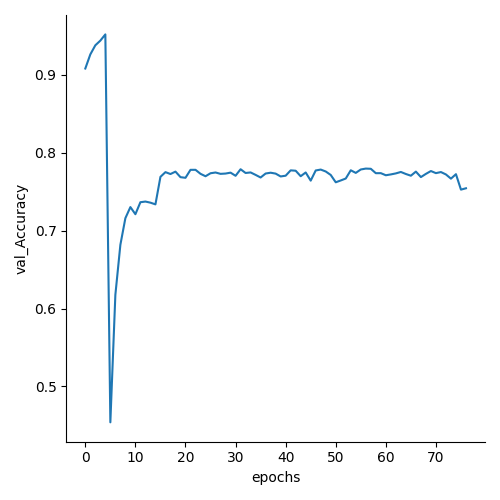
\includegraphics[height=5cm]{../Plots/models_02_m2s/val_Accuracy.png}
        \caption{\label{fig:figure6} Normal Data: MNIST to SVHN Network with TF between}
    \end{figure}
    Bei weniger Daten hat dasselbe Netz dann nur noch eine Accuracy von 56.6\%. Diese kann 
    durch verschiedene Epochenanzahlen in den Layern auf 68.4\% erhöht werden, 
    indem die Convolutionlayer mehr Epochen haben als die anderen Layer.
    Zum Vergleich: 
    Das Netz, welches SVHN löst ohne Kaskadierung hat 82.3\% und mit Kaskadierung 
    72.9\%. Das heißt, dass TF auch in diesem Fall nichts für die Performanz 
    der Netze bringt. 
    Wenn dann aber die Trainaccuracy mit der Validationaccuracy vergleicht kommt 
    dabei raus, dass beide Netze schlecht generalisieren. Dies liegt aber an den 
    absichtlich wenigen Trainingsdaten. Mit TF ist der Unterschied zwischen den 
    beiden Werten mit 21\% etwas geringer als ohne mit 26\%.
    Bei viel weniger Trainingsdaten sieht es noch schlimmer aus: 
    \begin{figure}[htpb]
        \includegraphics[height=5cm]{../Plots/models_02_m2s/VLAccuracy.png}
        \includegraphics[height=5cm]{../Plots/models_02_m2s/VLval_Accuracy.png}
        \caption{\label{fig:figure7} Very less Data: Vergleich zwischen ACC und Val-ACC mit TF}
    \end{figure}
    Der Unterschied ist bei etwa 40\%. Wenn kein TF gemacht wird, ist das Ergebnis folgendes: 
    \begin{figure}
        \includegraphics[height=5cm]{../Plots/models_02_m2s/VLwoAccuracy.png}
        \includegraphics[height=5cm]{../Plots/models_02_m2s/VLwoval_Accuracy.png}
        \caption{\label{fig:figure8} Very less Data: Vergleich zwischen ACC und Val-ACC ohne TF}
    \end{figure}
    Daraus folgt, dass das Netz ohne TF immer noch besser ist als mit. 
    Die Vermutung ist, dass diese beiden Datensätze doch etwas zu weit 
    auseinander liegen für TF.

\subsection{Overfitting auf MNIST und SVHN}
    Das Target-Dataset ist hier ebenfalls klein, also bei etwa 7000 Samples. 
    Das Netz ist bereits vorgestellt worden im zweiten Teil von dem 
    Abschnitt Keras Netzwerke. Hier wurden allerdings im zweiten MaxPool-Layer 
    zwei Epochen trainiert und im Dense zwanzig. 
    \begin{table}[h!]
        \begin{center}
            \caption{TF im Layer vorn bis hinten}
            \label{tab5:Table}
            \begin{tabular}{l|l|l}
                Bestes & Epoche & Endergebnis \\
                70.7\% & 14 & 58.1\% \\
                63.7\% & 13 & 62.1\% \\
                69.9\% & 14 & 61.3\% \\
                63.9\% & 14 & 54.1\% \\
                63.2\% & 16 & 57.2\% \\
            \end{tabular}
        \end{center}
    \end{table}
    Der erste Eintrag hier ist ohne TF. Es hat zwar die beste Performanz in der Spitze, 
    aber es wird danach deutlich schlechter. Es kam zu Overfitting auf dem SVHN-Datensatz. 
    TF verringert dieses Problem auf dem Targetdatensatz, wenn es auf 
    den Sourcedaten nicht zu Overfitting kommt. Damit dies nicht passiert, ist es sinnvoll das 
    SourceNet möglichst klein zu halten. 

\subsection{Weitere Netze}
    Es wurde noch Conv8Epochs, Dropout, BatchNorm und light svhn-solver durchgetestet. 
    Bei allen war es das Gleiche, dass sie ohne TF besser sind als mit. Zum Vergleich, wie 
    diese Netze einander gegenüber abschneiden, hier die Plots in der oben genannten Reihenfolge: 
    \begin{figure}[htpb]
        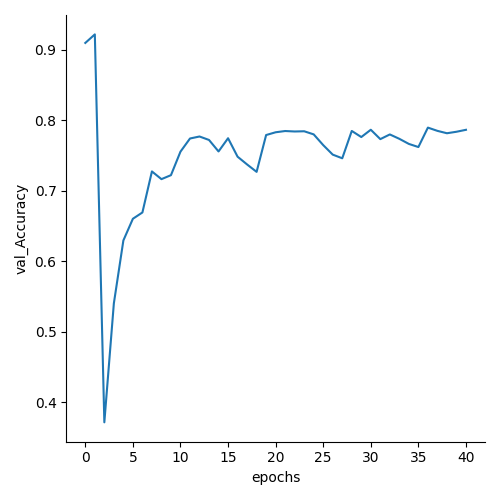
\includegraphics[height=5cm]{../Plots/models_03_C8E/val_Accuracy.png}
        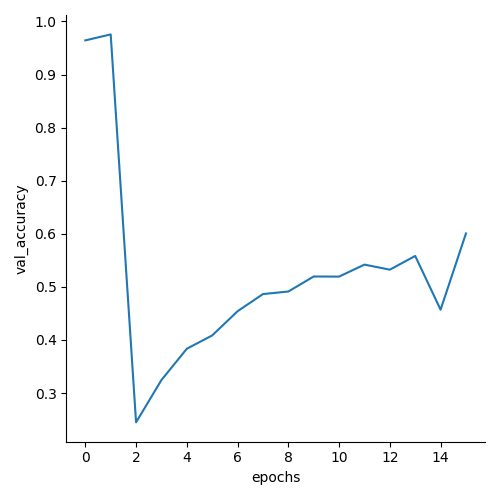
\includegraphics[height=5cm]{../Plots/models_02_DrO/val_Accuracy.png}
        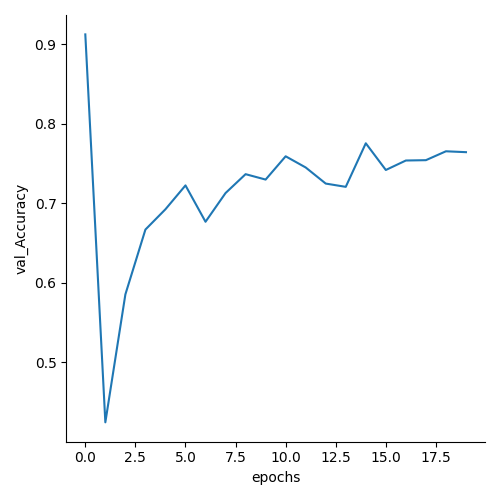
\includegraphics[height=5cm]{../Plots/models_02_BtN/val_Accuracy.png}
        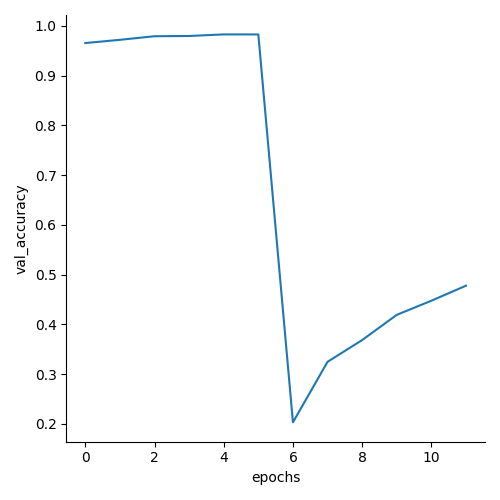
\includegraphics[height=5cm]{../Plots/models_01_Sce/val_Accuracy.png}
        \caption{\label{fig:figure9} Normal Data: Val-ACC Vergleich zwischen 4 Netzen}
    \end{figure}

    Da das Conv8Epochs Netz das Beste ist, wird dieses noch eingehender betrachtet. 
    Dieses Netz hat folgende Werte mit dem komplettem Datensatz: 
    \begin{figure}[htpb]
        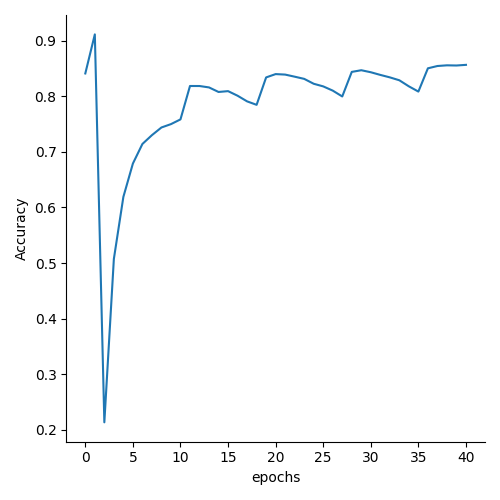
\includegraphics[height=5cm]{../Plots/models_03_C8E/Accuracy.png}
        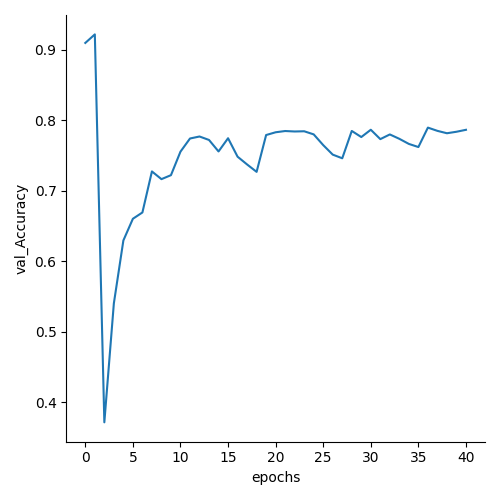
\includegraphics[height=5cm]{../Plots/models_03_C8E/val_Accuracy.png}
        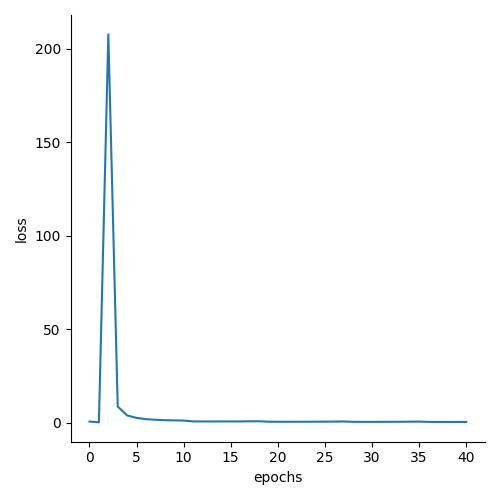
\includegraphics[height=5cm]{../Plots/models_03_C8E/loss.png}
        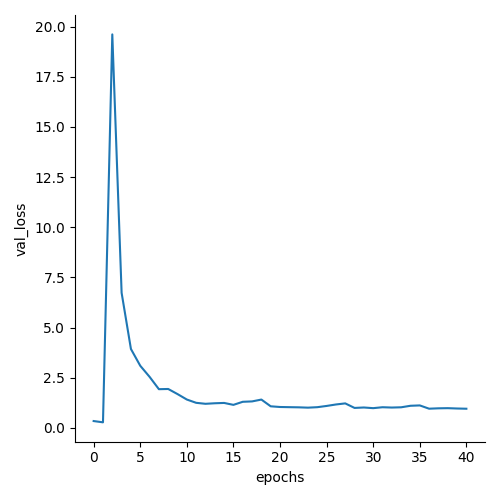
\includegraphics[height=5cm]{../Plots/models_03_C8E/val_loss.png}
        \caption{\label{fig:figure10} Normal Data: Alle Werte des Conv8Epochs}
    \end{figure}

    Das mit viel weniger Daten hat die Werte: 
    \begin{figure}[htpb]
        \includegraphics[height=5cm]{../Plots/models_03_C8E/VLAccuracy.png}
        \includegraphics[height=5cm]{../Plots/models_03_C8E/VLval_Accuracy.png}
        \includegraphics[height=5cm]{../Plots/models_03_C8E/VLloss.png}
        \includegraphics[height=5cm]{../Plots/models_03_C8E/VLval_loss.png}
        \caption{\label{fig:figure11} Very less Data: Alle Werte des Conv8Epochs}
    \end{figure}

    Zum Vergleich den ganzen Kram ohne TF: 
    \begin{figure}[htpb]
        \includegraphics[height=5cm]{../Plots/models_03_C8E/VLwoAccuracy.png}
        \includegraphics[height=5cm]{../Plots/models_03_C8E/VLwoval_Accuracy.png}
        \includegraphics[height=5cm]{../Plots/models_03_C8E/VLwoloss.png}
        \includegraphics[height=5cm]{../Plots/models_03_C8E/VLwoval_loss.png}
        \caption{\label{fig:figure12} Very less Data: Alle Werte des Conv8Epochs ohne TF}
    \end{figure}
    Auch hier bleibt es gleich, dass TF keinen Unterschied macht zwischen vielen oder wenigen 
    Target-Daten. 
